\documentclass{article}
\usepackage[utf8]{inputenc} % Accept raw UTF-8 (é, è, à, ç, …) in the source
\usepackage[T1]{fontenc}    % Render and encode accents as single glyphs (clean PDF copy-paste)
\usepackage{graphicx}       % Required for inserting images
\usepackage{url}            % Typeset the repository URL cleanly
\usepackage[round]{natbib}  % Author-year bibliography style (matches in-text format)

\title{From centroid to entrance: a global assessment of POI access locations for accessibility}
\author{Pierre-Léo Bourbonnais, Yannick Brosseau, Catherine Morency (Polytechnique Montréal)}
\date{April 2026}

\begin{document}

\maketitle

\section{Introduction}

Points of interest (POIs) and residential locations serve as origins and destinations
when estimating travel demand and modelling behaviour. The
underlying data come from travel surveys, property registries,
GPS traces and, increasingly, OSM, which acts both as a
crowdsourced database and as an openly licensed container for
license-compatible authoritative datasets. When footprints are
available, most researchers approximate each POI by the centroid
of its polygon (or the parcel where no building is mapped). On
small single-purpose buildings this is acceptable; on larger and
multi-building sites the centroid can misrepresent the access
point by hundreds of metres---sometimes kilometres---which is not
negligible for walking or first-/last-mile transit.

Entrances can be tagged explicitly via OSM \texttt{entrance=*}
(\texttt{main}, \texttt{customers}, \texttt{home}, \texttt{yes},
\ldots) but remain sparsely mapped outside a few well-covered
regions. Large sites usually expose several entrances with
distinct functions---main, visitors, employees, deliveries,
emergency---each with its own accessibility profile. Precise
access points matter most for paratransit and wheelchair users,
transit riders for whom the stop-to-door segment dominates total
travel time, cyclists seeking secure parking, and routing engines
including autonomous taxis, for which curbside drop-off precision
is a safety and usability requirement.

A growing literature characterises the completeness and
positional accuracy of OSM buildings and POIs (Haklay, 2010;
Girres \& Touya, 2010; Fan et al., 2014; Herfort et al., 2023;
Klinkhardt et al., 2023) and shows that entrance-level detail
changes transit catchments (Gutiérrez \& García-Palomares,
2008; El-Geneidy et al., 2014), wheelchair routing (Neis \&
Zielstra, 2014), and curbside outcomes for autonomous vehicles
(Hunter et al., 2024; Wang et al., 2025). The \texttt{entrance=*}
tag itself remains a blind spot: Hu et al.\ (2021) found only
\(\approx\)60 tagged buildings in their entire London extract.
Our prior work (Bourbonnais et al., 2026) validated 1{,}034 POIs
from five Québec household travel surveys and observed median
positional errors around 20\,m across OSM, Overture Maps, the
Québec Property Registry and Google Places, with long tails
dominated by university campuses and hospital complexes; it
explicitly flagged the centroid-vs-entrance comparison as open.
To our knowledge, no study yet quantifies \texttt{entrance=*}
coverage at scale, nor the cost of substituting a centroid for
an entrance. We quantify that gap on a worldwide random sample
of POIs by comparing centroid baselines to the nearest tagged
entrance, and show how entrances can be mapped to support
walking, cycling, transit and autonomous-vehicle use cases.

\section{Methodology}

The study is a global exploratory analysis. POIs are coded
along four axes: building footprint
present or not; single- vs.\ multi-building site;
\texttt{entrance=*} present or not; and specificity of the
entrance tag (values other than \texttt{yes}). Coverage extends
beyond buildings to polygon-mapped sites without a unique
footprint---e.g.\ university campuses, large factory areas, or
sport pitches---where the area polygon itself supplies the
centroid baseline.

\paragraph{Two complementary sampling strategies.} A global pass
tessellates the world into $10\times10$\,km cells over GHS-POP
and GHS-BUILT-V (Joint Research Centre) and draws cells with
probability proportional to a \emph{blended} mix of population
and built volume (default $\alpha=0.5$). The built-volume term
prevents low-residency but high-activity fabric---campuses,
industrial parks, transport hubs---from being under-sampled by a
purely population-weighted draw. The current round is purely
random, which under-samples the large multi-building sites where
the centroid proxy is most misleading. A complementary targeted
pass---the analyst supplies a precise point or OSM
node/way/relation---will characterise the upper tail on a curated
list of large sites; both passes share the same pipeline.

\paragraph{Reference entrances and centroid baselines.} Reference
entrances are established from open and proprietary street-level
imagery (Mapillary, KartaView, Panoramax, Google Street View,
and the Chinese Baidu Panorama and AMap services) and, where
available, architectural or wayfinding plans. A non-trivial share
of randomly selected POIs are rejected at this stage---most often
because aerial and street-level imagery do not let the analyst
confidently locate entrances, or because the underlying tag is
obsolete (e.g.\ a closed shop). Four centroid baselines are
compared against each OSM entrance: parcel, main-building, and
all-buildings centroids where a footprint exists, and the
area-polygon centroid for sites without a unique footprint
(campuses, factory areas, sport pitches).

\paragraph{Distance metrics and persisted measurements.} The
analyst draws a polyline on the focus map---a single Euclidean
segment, or a multi-vertex trace along sidewalks/desire lines
where mapped paths are missing. Each polyline is persisted with
its geodesic length, walking duration at a configurable speed,
coordinates, an analyst-supplied \emph{purpose} (nearest entrance,
main entrance, transit stop, off-street parking, driving road,
and walking/cycling/driving network combinations) and
\emph{entrance class} (\texttt{main}, \texttt{customers},
\texttt{home}, \texttt{emergency}, service-employees,
service-delivery, \texttt{garage}, or one of four centroid
baselines: parcel, main-building, all-buildings, or area).

\paragraph{Pipeline and OSM contributions.} The pipeline is a Rust
backend over PostgreSQL/PostGIS, fed by Overpass for OSM
features, with a React/MapLibre review interface; all code, the
sampled POI list and computed metrics are
released under an open licence. OSM edits made during the
analysis to add missing entrances and pedestrian-access
geometry (footpaths and connecting paths) for the selected POIs
carry the \texttt{\#StateOfTheMap2026} and
\texttt{\#EntranceAnalysis} hashtags in their changeset
comments, so every contribution is traceable. Repository:
\url{https://github.com/chairemobilite/stateofthemap2026}
(translations, drafting and parts of the pipeline were assisted by Anthropic
Claude Opus 4.6 and 4.7; all data, methods and
findings remain the authors').

\section{Review interface}

The review service is a single-page Rust/React/MapLibre
application (Figure~\ref{fig:ui}) with four screens. \emph{Sampling}
draws a candidate $10\times10$\,km cell or accepts a custom
anchor and previews its weights. \emph{Kept bboxes} lists
accepted cells and their POI inventory. \emph{POI focus} centres
the map on a selected POI, lets the analyst draw, classify and
persist measurements (purpose $\times$ entrance class) over OSM
buildings and entrances inside a configurable focus radius, and
provides right-click deeplinks to the imagery providers listed
above and to the OSM iD editor. \emph{Stats}
aggregates min, max, mean and median length and walking duration
over all persisted measurements, grouped pairwise by
\texttt{measurement\_type}, \texttt{entrance\_type}, and
\texttt{start\_origin}.

\begin{figure}[h]
\centering
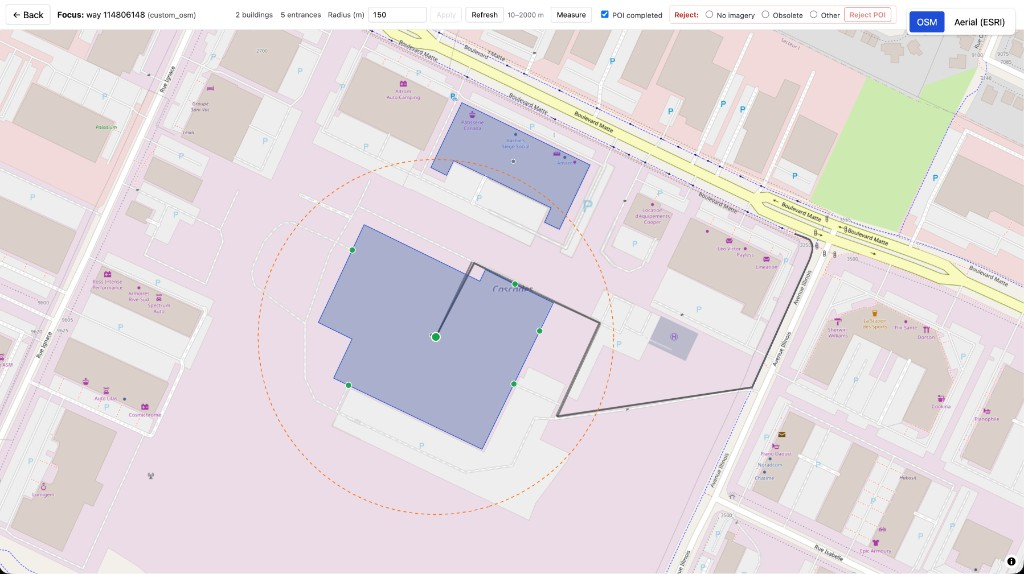
\includegraphics[width=0.95\linewidth]{figures/ui_focus.png}
\caption{POI focus screen for one POI: building polygons,
entrance nodes (green), the configurable focus radius (orange),
and an analyst-drawn polyline from the building centroid to the
nearest tagged entrance.}
\label{fig:ui}
\end{figure}

\section{Preliminary findings}

The initial pass is a 100\% random draw of $\approx$25 POIs,
predominantly in North America (Figure~\ref{fig:world}), yielding
140 measurements. For each POI we pair the centroid-anchored
polyline with the nearest tagged-entrance polyline drawn to the
same target and report the per-POI difference; a positive value
means the centroid proxy yields a longer walk than the real
entrance. We aggregate by target family across all centroid
types (area, main-building, multi-building).

\begin{figure}[h]
\centering
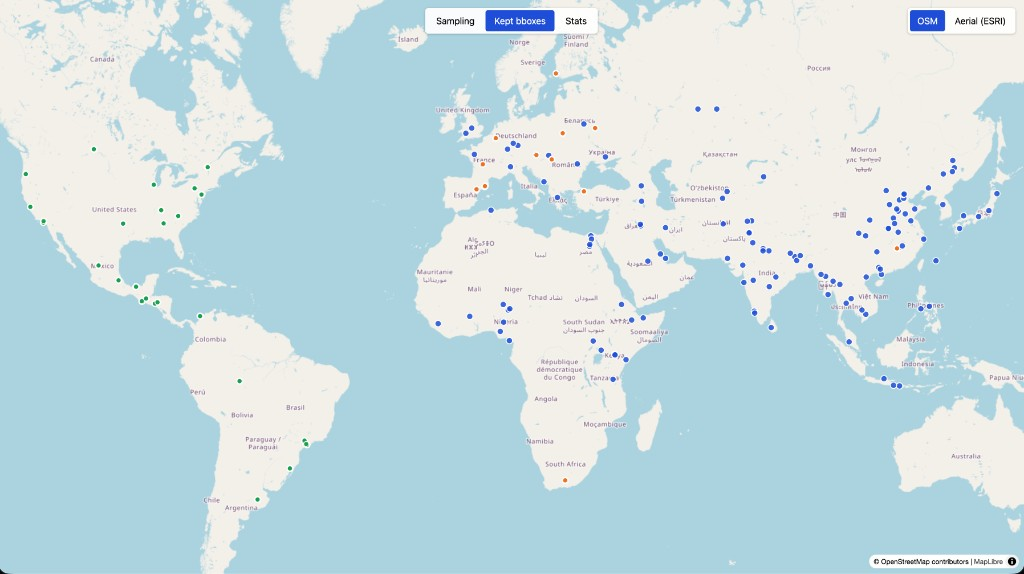
\includegraphics[width=0.95\linewidth]{figures/kept_bboxes_world.png}
\caption{Random initial sample: kept $10\times10$\,km cells
worldwide (green: completed POI; orange: in progress; blue:
not yet started).}
\label{fig:world}
\end{figure}

Across the 25 paired observations, 24 are positive (single
$-$8\,m exception). The pooled difference is $+$16\,m median,
$+$80\,m max for distance to nearest road network ($n=$15); $+$37\,m
median, $+$92\,m max for distance to nearest transit stop ($n=$10).

\textbf{These are preliminary figures from a small random draw,
not final results.} The full paper will combine a substantially
larger random sample, a targeted pass on large multi-building
and area-coded sites, and the regional Québec field-validated
analysis, all through the same pipeline.

% In-text citations are still typeset manually in author-year form;
% \nocite forces the bibliography to print the Part 1 entries listed
% in bibliography.bib so they appear in the PDF.
\bibliographystyle{plainnat}
\nocite{Bourbonnais2026, Herfort2023, Hu2021, Klinkhardt2023,
        Haklay2010, Girres2010, Fan2014, Moradi2023,
        Gutierrez2008, Biba2010, ElGeneidy2014, Neis2014,
        Hunter2024, Wang2025}
\bibliography{bibliography}

\end{document}
